\documentclass{article}
\usepackage{graphicx}
\usepackage{multicol}

\usepackage{authblk} % For author affiliations
\usepackage[margin=1in]{geometry}
\usepackage{float}

\title{Investigation of Self Supervised Learning with Passive Acoustic Data}
\author{Gary Huntress}

\affil{NUWCDIVNPT, Code 4542}
\begin{document}
\maketitle
\begin{abstract}
This is a preliminary investigation and proof of concept to use self-supervised learning (SSL) with acoustic data.  SSL is used to pre-train a foundational model such that it learns common features of the data.  This is done using a \textit{"pretext"} task and unlabeled data.  A corpus of passive acoustic data was obtained from NOAA.  A very simple SSL pretext task was defined.  The model was trained and validated on a subset of the NOAA data and then tested with \textit{gold} data from an unrelated passive acoustic dataset.  ROC/AUC testing demonstrated the sucess of the approach.  


\end{abstract}
 

% switch to two-column layout
\begin{multicols}{2}
\section{Introduction}
There are many techniques and approaches that can be used for successful machine learning.  One of the most successful approaches is Supervised Classification.  A common example is to assign a label (e.g. "cat", "dog") to an object in an image.  In order to be successful, an ML model requires a large amount of pre-labeled images.  A major drawback of Supervised Classification is that labeling commonly requires human effort and this is expensive.   

  

\section{Self-Supervised Classification (SSL)}
Many organizations have large archives of domain specific data and a desire to classify objects in images or events in audio.  The goal of SSL is to extract  features of the data, without overt labels.  The method relies on the definition of a \textit{pretext} task unrelated to the downstream supervised task.  These labels are in essence "free".

Consider the pretext task depicted in figure 1.  Assume that the ultimate goal is to classify objects in images.  A large set of images exist without labels. We need to define and construct a supervised learning task with known inputs and outputs.  This is defined as follows:
\begin{itemize}
\item Select a random picture from the dataset
\item Place a 3 x 3 grid randomly onto the picture.  This defines 9 small patches
\item The center patch is always the "anchor" 
\item Randomly select one of the remaining 8 patches 
\item The input to the pretext model is the pair (anchor, random patch).  This could be implemented with standard CNN or dense layers, or a pretrained model.
\item The output to the pretext model is the corresponding number 1-8 of the random patch.  This would be typically implemented as a standard softmax.

\end{itemize}
The model is then trained extensively on the entire dataset.  This is possible because the random training patches obtained when an image is re-used are very weakly correlated.

The key takeaway from this task is that if this pretext model trains successfully, it must have learned the representative features in the underlying images, without any overt labels.  In the figure, if you assume the model trained well, then it must have learned the features of the cat and the spatial relationship between the face and ear (lower left pair)

Once a pretext model is trained, it can then be used on the downstream task.  This will usually be a traditional supervised learning task that will still require high quality labeled data (there is no free lunch).  But this could be reduced by 95\% or more.

\end{multicols}
\begin{figure}[H]
  \centering
  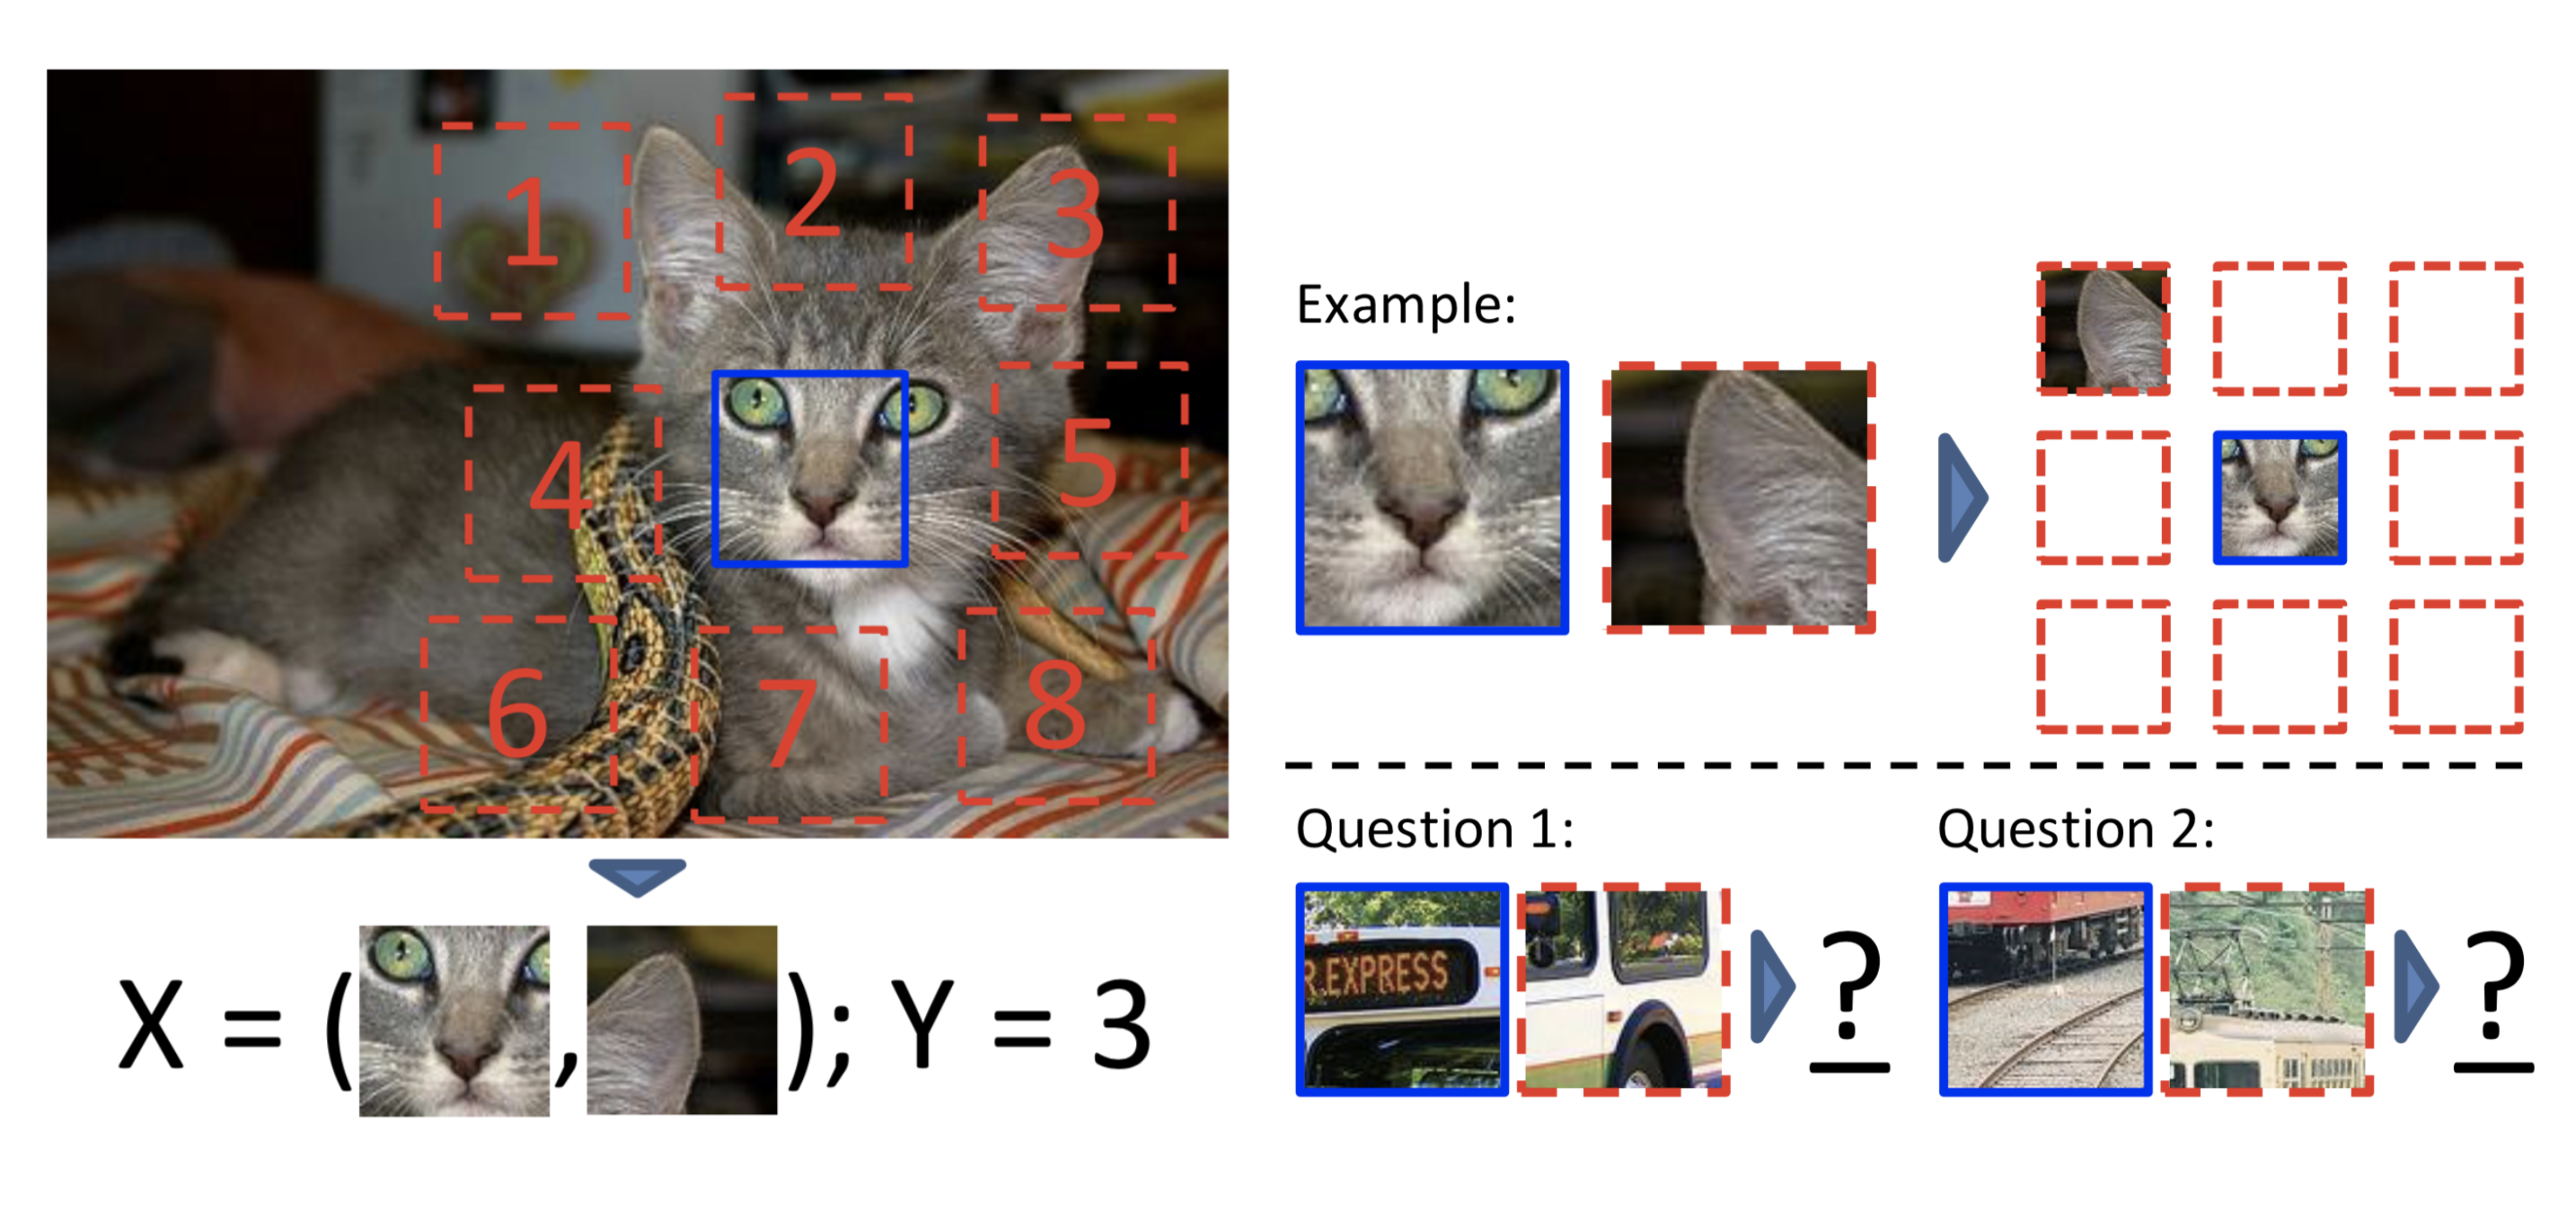
\includegraphics[width=.8\textwidth]{self-sup-by-relative-position.png}  
  \caption{Pretext task example.}
  \label{fig:example}
\end{figure}
\begin{multicols}{2}
 
\section{Data}
NOAA\cite{example1} maintains a public archive of passive acoustic data.  The data files vary in both temporal and geographic locations.  The data is known to include many acoustic features such as multiple whale species, shipping, sonar, explosions, and varied background noise.  Each data file is approximately 3 hours in duration with a sample rate of 96KHz.   It is not feasible to obtain the entire 400+ TB archive.  The primary dataset used for experimentation is the CIO1 subset of the "Sanctuary Sound" archive.  Data was collected off the north coast of Santa Rosa Island CA across multiple months.  Approximately 3000 data files (9000 hours) were obtained.   

Each raw file is decomposed into "clips" approximately 10 seconds in duration.  

As a proof of concept a train/test split was produced of 15k and 15000 files.



\section{Methodology}
In order to train an SSL model, a "pretext" task is defined that leverages the unlabled data on hand (the acoustic time series) to produce usable pseudo labels inherent in the data itself.  The proxy task used was as follows:

\begin{itemize}
\item Select hyperparameter for the length of the sub-clip N 
\item Draw two random audio clips A and B
\item Draw two random index values
\item Produce subclips A[idx:idx+N] and B[idx:idx+N]
\item Increase the difficulty by zeroing out an interval of each clip
\item Flip a coin to produce a third clip X derived from either A or B
\item Train the model on this supervised [ABX] input and the known coin flip choice.
\end{itemize}

The input to the model is the concatenation of two known random samples A and B, and a third clip from either A or B.   This is shown in Figure 2.
A simple 6 layer 1D CNN network was built with Keras.  The model has a single sigmoid output.  A dropout layer was used in the model to provide minimal regularization.  This is in addition to the zeroing of intervals within each data sample.  The model consisted of approximately 12.5M parameters.   The model was trained for 25 epochs.

\begin{figure}[H]
  \centering
  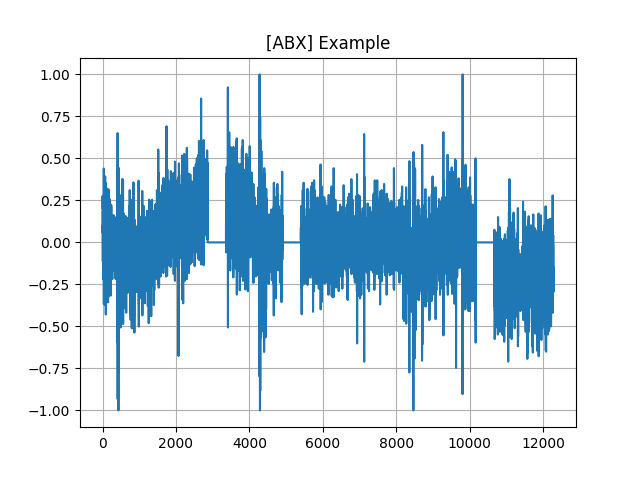
\includegraphics[width=.5\textwidth]{abx_example.png}  
  \caption{One input training example.}
  \label{fig:example}
\end{figure}

\section{Results}
A ROC curve is used to summarize the performance of a binary classifier.  A completely random classifier is unable to do better than a 50/50 guess.  This is depicted on a ROC curve as the red dashed diagonal line.  Better performance moves the curve up and to the left, toward the ideal perfect classifier that has 100\% true positives.  The results of three epochs are shown.  Looking closely you can see that the baseline model trained on one epoch lies almost exactly on the 50/50 line.  Model checkpoints 4 and 5 have performance about 80\%.
\begin{figure}[H]
  \centering
  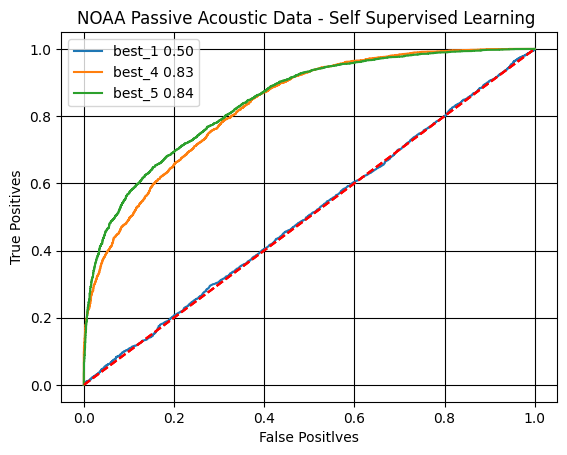
\includegraphics[width=.5\textwidth]{roc_auc.jpg}  
  \caption{ROC Curve.}
  \label{fig:example}
\end{figure}
\section{Discussion}
It trained and validated well. Though it did appear to reach diminishing returns at about 80% 
 
It tested well on gold data from another dataset.
Show improvement over each epoch

Maybe this is still too easy.  It's possible this model just learned background features and not full representations.


\section{Conclusion}
There is every indidation that this model has learned sufficient acoustic features.  This approach may be extensively broadened to include orders of magnitude more data, more complex models (e.g. 1D CNN).

\begin{itemize}
\item ABX with more augmentation
\item ABX with spectrograms
\item "One of Four", pick which of the four is the odd candidate
\item Which time series goes with which spectrum?
\end{itemize}

Future tasks include exploration of various downstream tasks (e.g. whale classification).  


% Example of citing references
\begin{thebibliography}{9}
\bibitem{example1} NOAA Passive Acoustic Dataset https://www.ncei.noaa.gov/products/passive-acoustic-data
\bibitem{example2} Discussion of Self Supervised Learning https://arxiv.org/abs/2304.12210
\end{thebibliography}

\end{multicols}
 
\end{document}